\documentclass{article}

\usepackage[T1]{fontenc}    %Schriftart des Dokumentes
\usepackage[ngerman]{babel} %Dokumentensprache, hier Deutsch
\usepackage{amsmath, amssymb, stmaryrd} %mathematische Schriftzeichen
\usepackage{graphicx} %Einfügen von Grafiken
\usepackage{wrapfig}
\usepackage{bm}

\setlength{\parindent}{0pt} %Einrückung von Absätzen auf null gesetzt
\setlength{\parskip}{10pt} %Abstand zischen Absätzen auf 10pt gesetzt

\title{Versuch 21: Elektrolyse}
\author{Matthias Kuntz}
\date{26.09.2023}

\begin{document}

\maketitle

%-------------------------EINLEITUNG-------------------------
\section{Einleitung}

In diesem Versuch soll mithilfe von Elektrolyse die Faraday-Konstante bestimmt werden. Dazu betrachten wir zwei Versuchsteile: Im Ersten werden für die Elektrolyse zwei Kupferplatten in einer Kupfersulfat-Lösung verwendet und deren Massen davor und danach bestimmt. Beim zweiten Teil betrachten wir die elektrolytische Zersetzung von Wasser mithilfe eines Wasserzersetzungsapparats nach Hoffmann und messen das Volumen.

\subsection{Physikalische Grundlagen}

Als Elektrolyse bezeichnet man die Zersetzung eines Elektrolyts ausgelöst durch eine über zwei Elektroden angebrachte Spannung. Ein Elektrolyt ist dabei eine Flüssigkeit, deren Leitfähigkeit nicht auf freien Elektronen, sondern Ionen beruht. Im ersten Versuchsteil betrachten wir eine Kupfersulfatlösung (CuSO$_4$) mit zwei Kupferelektroden. Die Reaktionsgleichung der Elektrolyse ergibt sich zu:

\begin{equation}
    \text{CuSO}_4 \rightleftarrows \text{Cu}^{++} + \text{SO}_4^{--}
    \label{eq:elektrolyse1}
\end{equation}

Effizient wird bei diesem Vorgang also die positiv geladene Anode schwerer und die negativ geladene Kathode leichter. Der Betrag der Massedifferenz ist hierbei bei beiden gleich. Die von der Kathode abgeschiedene Masse $m$ lässt sich aus dem ersten Faradayschen Gesetz herleiten: 

\begin{equation}
    \begin{split}
        m = n M_{mol} = \frac{Q}{zF} M_{mol}
    \end{split}
    \label{eq:masse}
\end{equation}

Hierbei ist $n$ die von der Kathode abgeschiedene Stoffmenge, $M_{mol}$ die Molmasse von Kupfer, $Q$ die zwischen den Elektroden transportierte Ladung, $z$ die Wertigkeit der Ionen und $F$ die Faraday Konstante. Diese ist definiert als Elementarladung mal Avogadro-Konstante und gibt somit die Ladungsmenge, die durch einen Elektrolyten fließt, wenn sich $\frac{1}{z}$ Mol eines $z$-wertigen Stoffes an der Elektrode absetzt.

Die insgesamt transportierte Ladungsmenge lässt sich bestimmen als:

\begin{equation}
    Q=It
    \label{eq:Q}
\end{equation}

Im zweiten Versuchsteil betrachten wir die elektrolytische Zersetzung von mit Schwefelsäure gemischtes Wasser mit zwei Platin-Elektroden. Dabei treten die folgenden Reaktionen auf:

\begin{equation}
    \begin{split}
        2\text{H}^+ + 2e^- &\rightarrow \text{H}_2 \\
        2\text{OH}^- &\rightarrow \text{H}_2 \text{O} + \frac{1}{2} \text{O}_2 + 2e^-
    \end{split}
    \label{eq:elektrolyse2}
\end{equation}

An der Kathode, beschrieben durch die obere Reaktionsgleichung, bildet sich Wasserstoff und an der Anode, untere Gleichung, Sauerstoff. Wir können über die Stoffmenge folgende relation herleiten:

\begin{equation}
    n = \frac{Q}{zF} = \frac{V}{V_{mol}}
    \label{eq:F2}
\end{equation}

Hierbei ist $V$ das abgeschiedene Volumen von entweder Wasserstoff oder Sauerstoff unf $V_{mol}$ das jeweilige Molvolumen, welches über folgende Gleichung bestimmt werden kann:

\begin{equation}
    V_{mol} = \frac{p_0}{p} \frac{T}{T_0} V_{mol}^0
    \label{eq:Vmol}
\end{equation}

$T_0 = 273,15$K und $p_0 = 1013,25$mbar sind feste Werte, genauso wie das Molvolumen eines idealen Gases $V_{mol}^0 = 22,414 \frac{\text{l}}{\text{mol}}$. $T$ ist die Temperatur während der Elektrolyse und $p$ der Druck, welcher sich zusammensetzt aus dem äußeren Luftdruck $p_L$, dem Dampfdruck $p_D$ der verdünnten Schwefelsäure und dem hydrostatischen Druck $p_H$. Letzterer kann praktisch eliminiert werden, indem der Wasserspiegel den man misst auf eine Ebene mit dem Wasserreservoire gebracht wird. Somit bleiben $p_L$ und $p_D$. Der Sättigungsdruck des Elektrolyten wird mit 90\% des Sättigungsdampfdrucks reinen Wassers gleichgesetzt und wir erhalten:

\begin{equation}
    p= p_L - p_D^{\text{H$_2$SO$_4$}} = p_L - 0,9 \cdot p_D^{\text{H$_2$O}}
    \label{eq:druck}
\end{equation}

\subsection{Versuchsaufbau}

Eine genaue Skizze des Versuchsaufbaus ist auf der nächsten Seite im Messprotokoll zu sehen.

Im ersten Versuchsteil haben wir ein Gefäß mit der Kupfersulfatlösung, in die wir zwei Kupferplatten halten. An der Halterung ist für jede Platte ein Anschluss, sodass diese mit einer Stromquelle verbunden werden können. Im Stromkreis wird dann noch ein Schiebewiderstand eingeschlossen.

Im zweiten Versuchsteil benutzen wir einen Wasserzersetzungsapperat nach Hoffmann. Dieser besteht aus zwei senkrechten Röhren, die unten miteinander verbunden sind. Unten in den Rohren ist jeweils eine der Elektroden angebracht und ein Schlauch an der Verbindungsstelle führt zu einem höhenverstellbaren Behälter. Die Rohre und der Behälter sind mit der Schwefelsäure-Wasser-Mixtur befüllt. Im Behälter ist ein Thermometer angebracht und an den Röhren sind Skalen zum Bestimmen des Volumens in der Röhre.  

%---------------VERSUCHSPROTOKOLL MIT MESSDATEN---------------
\newpage

\section{Versuchsprotokoll mit Messdaten}

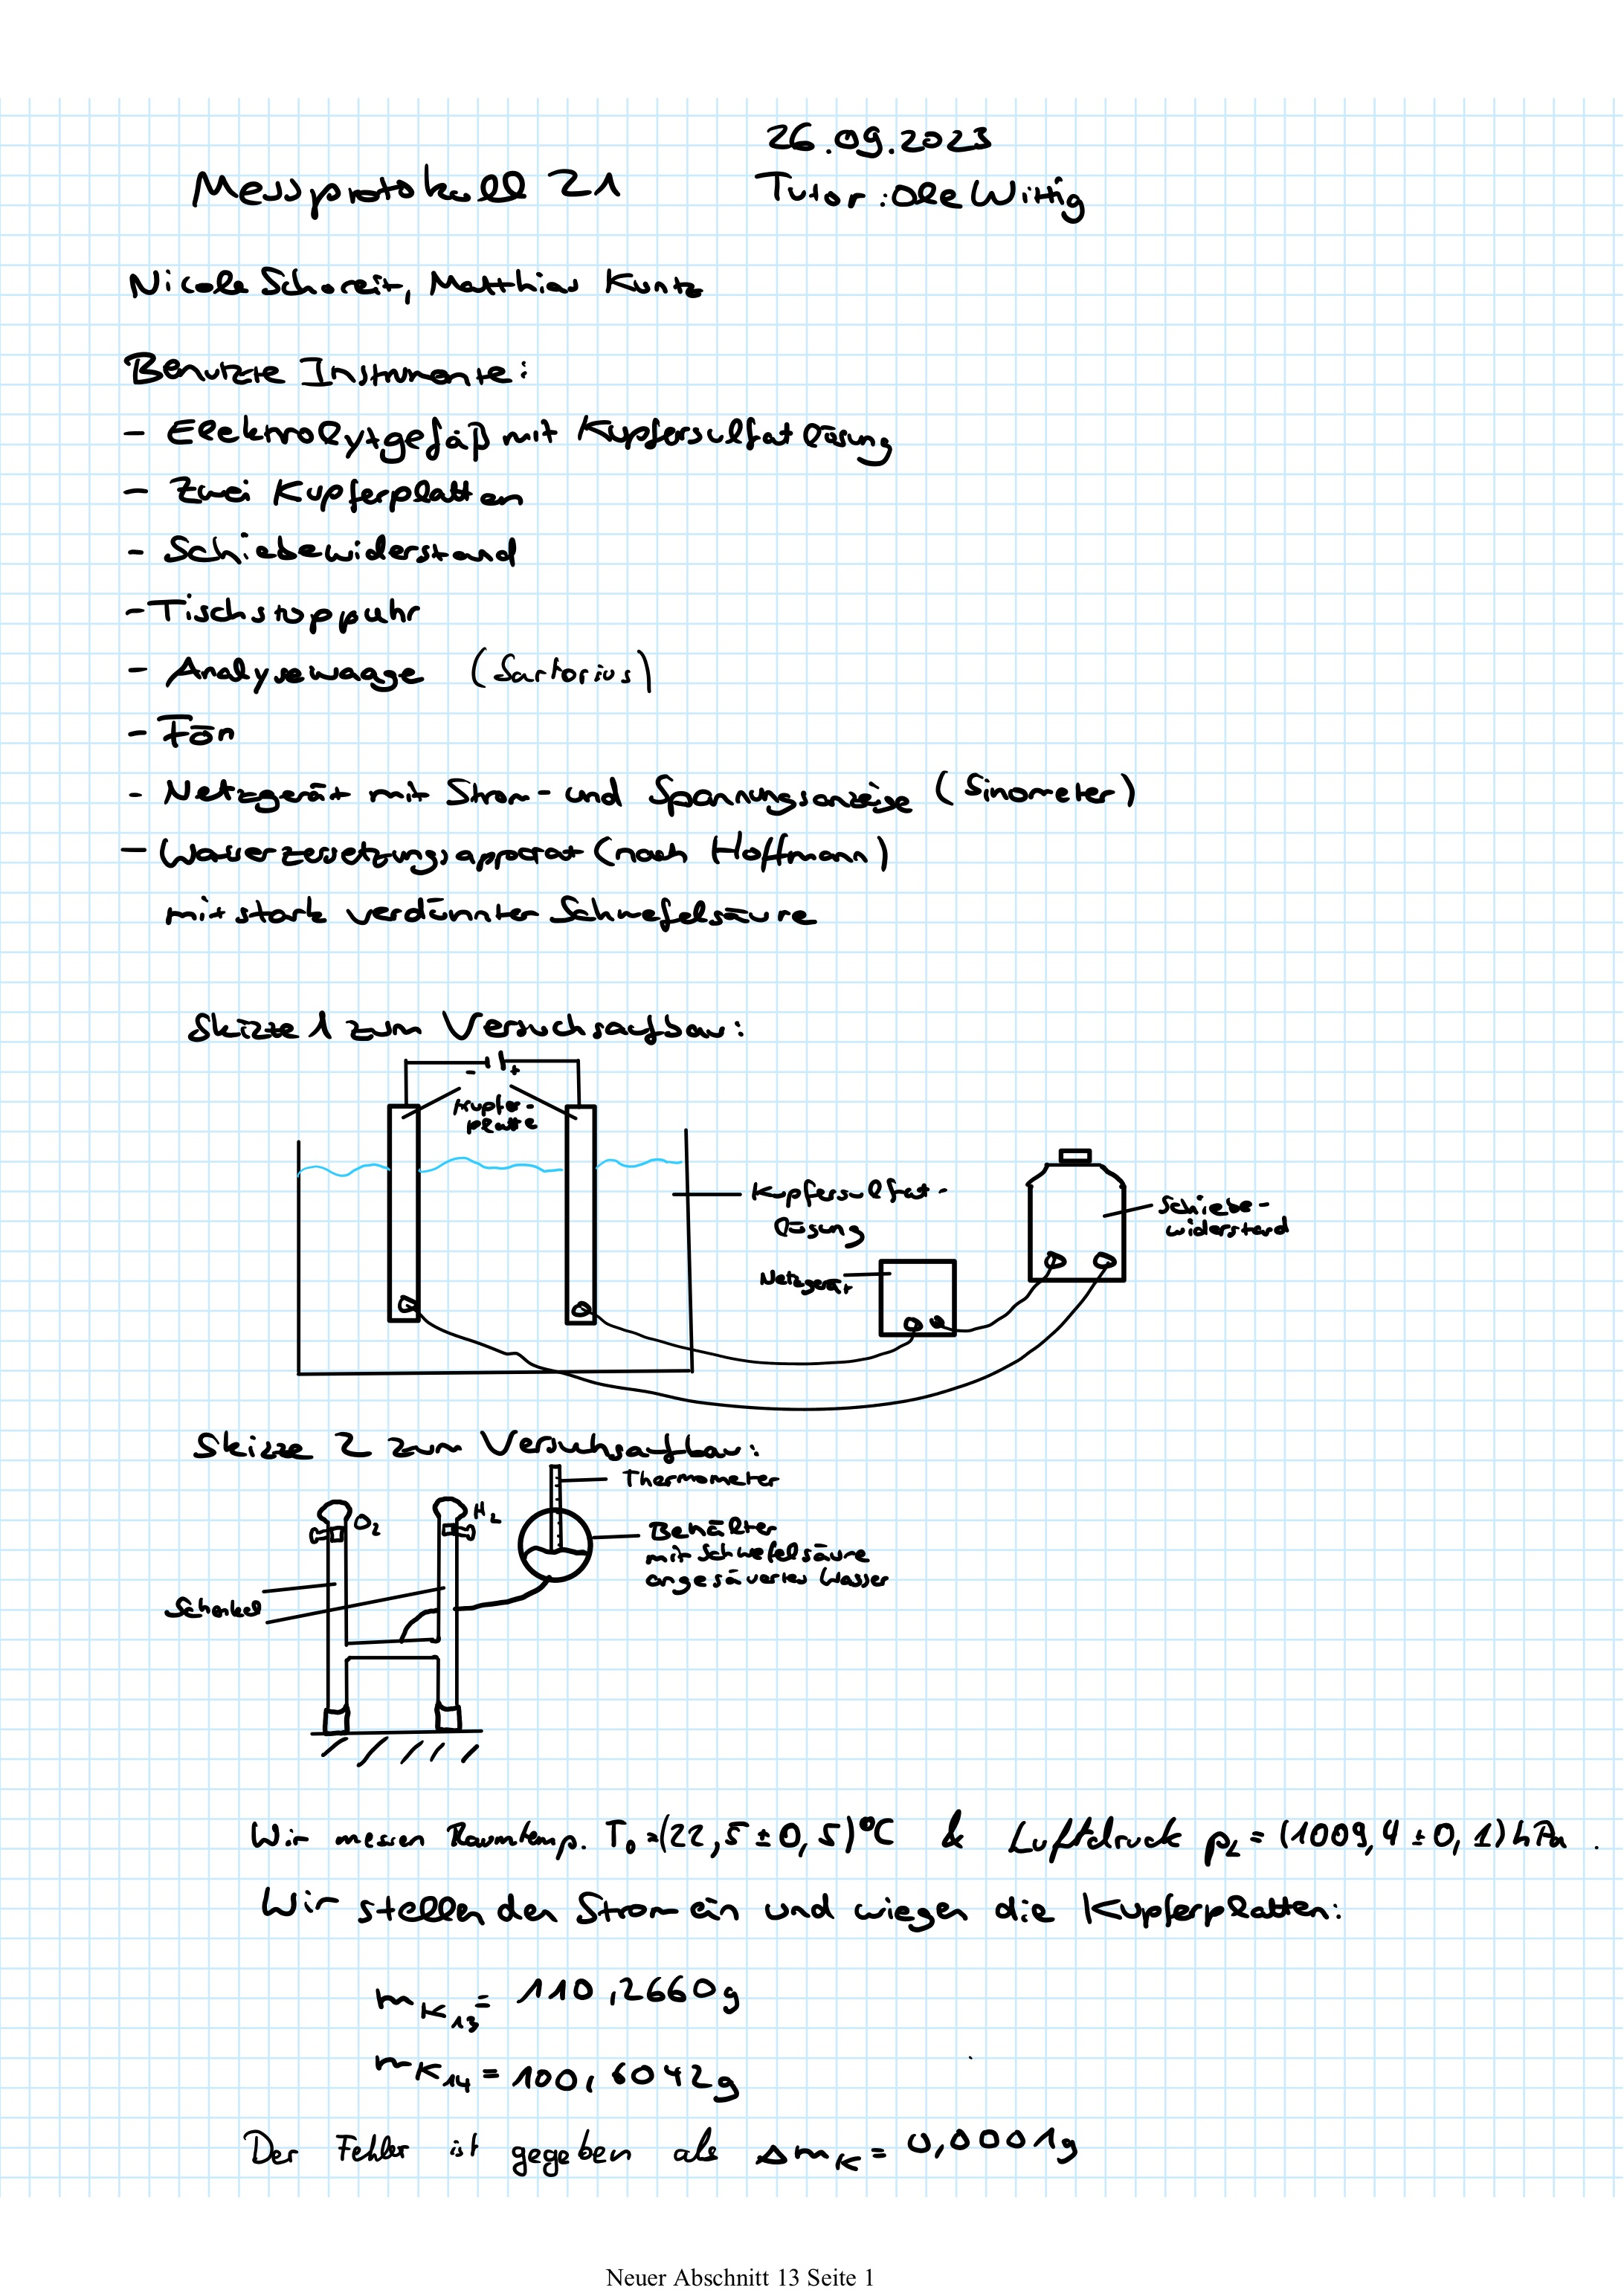
\includegraphics[width=\textwidth]{graphics/mess1.jpg}
\newpage
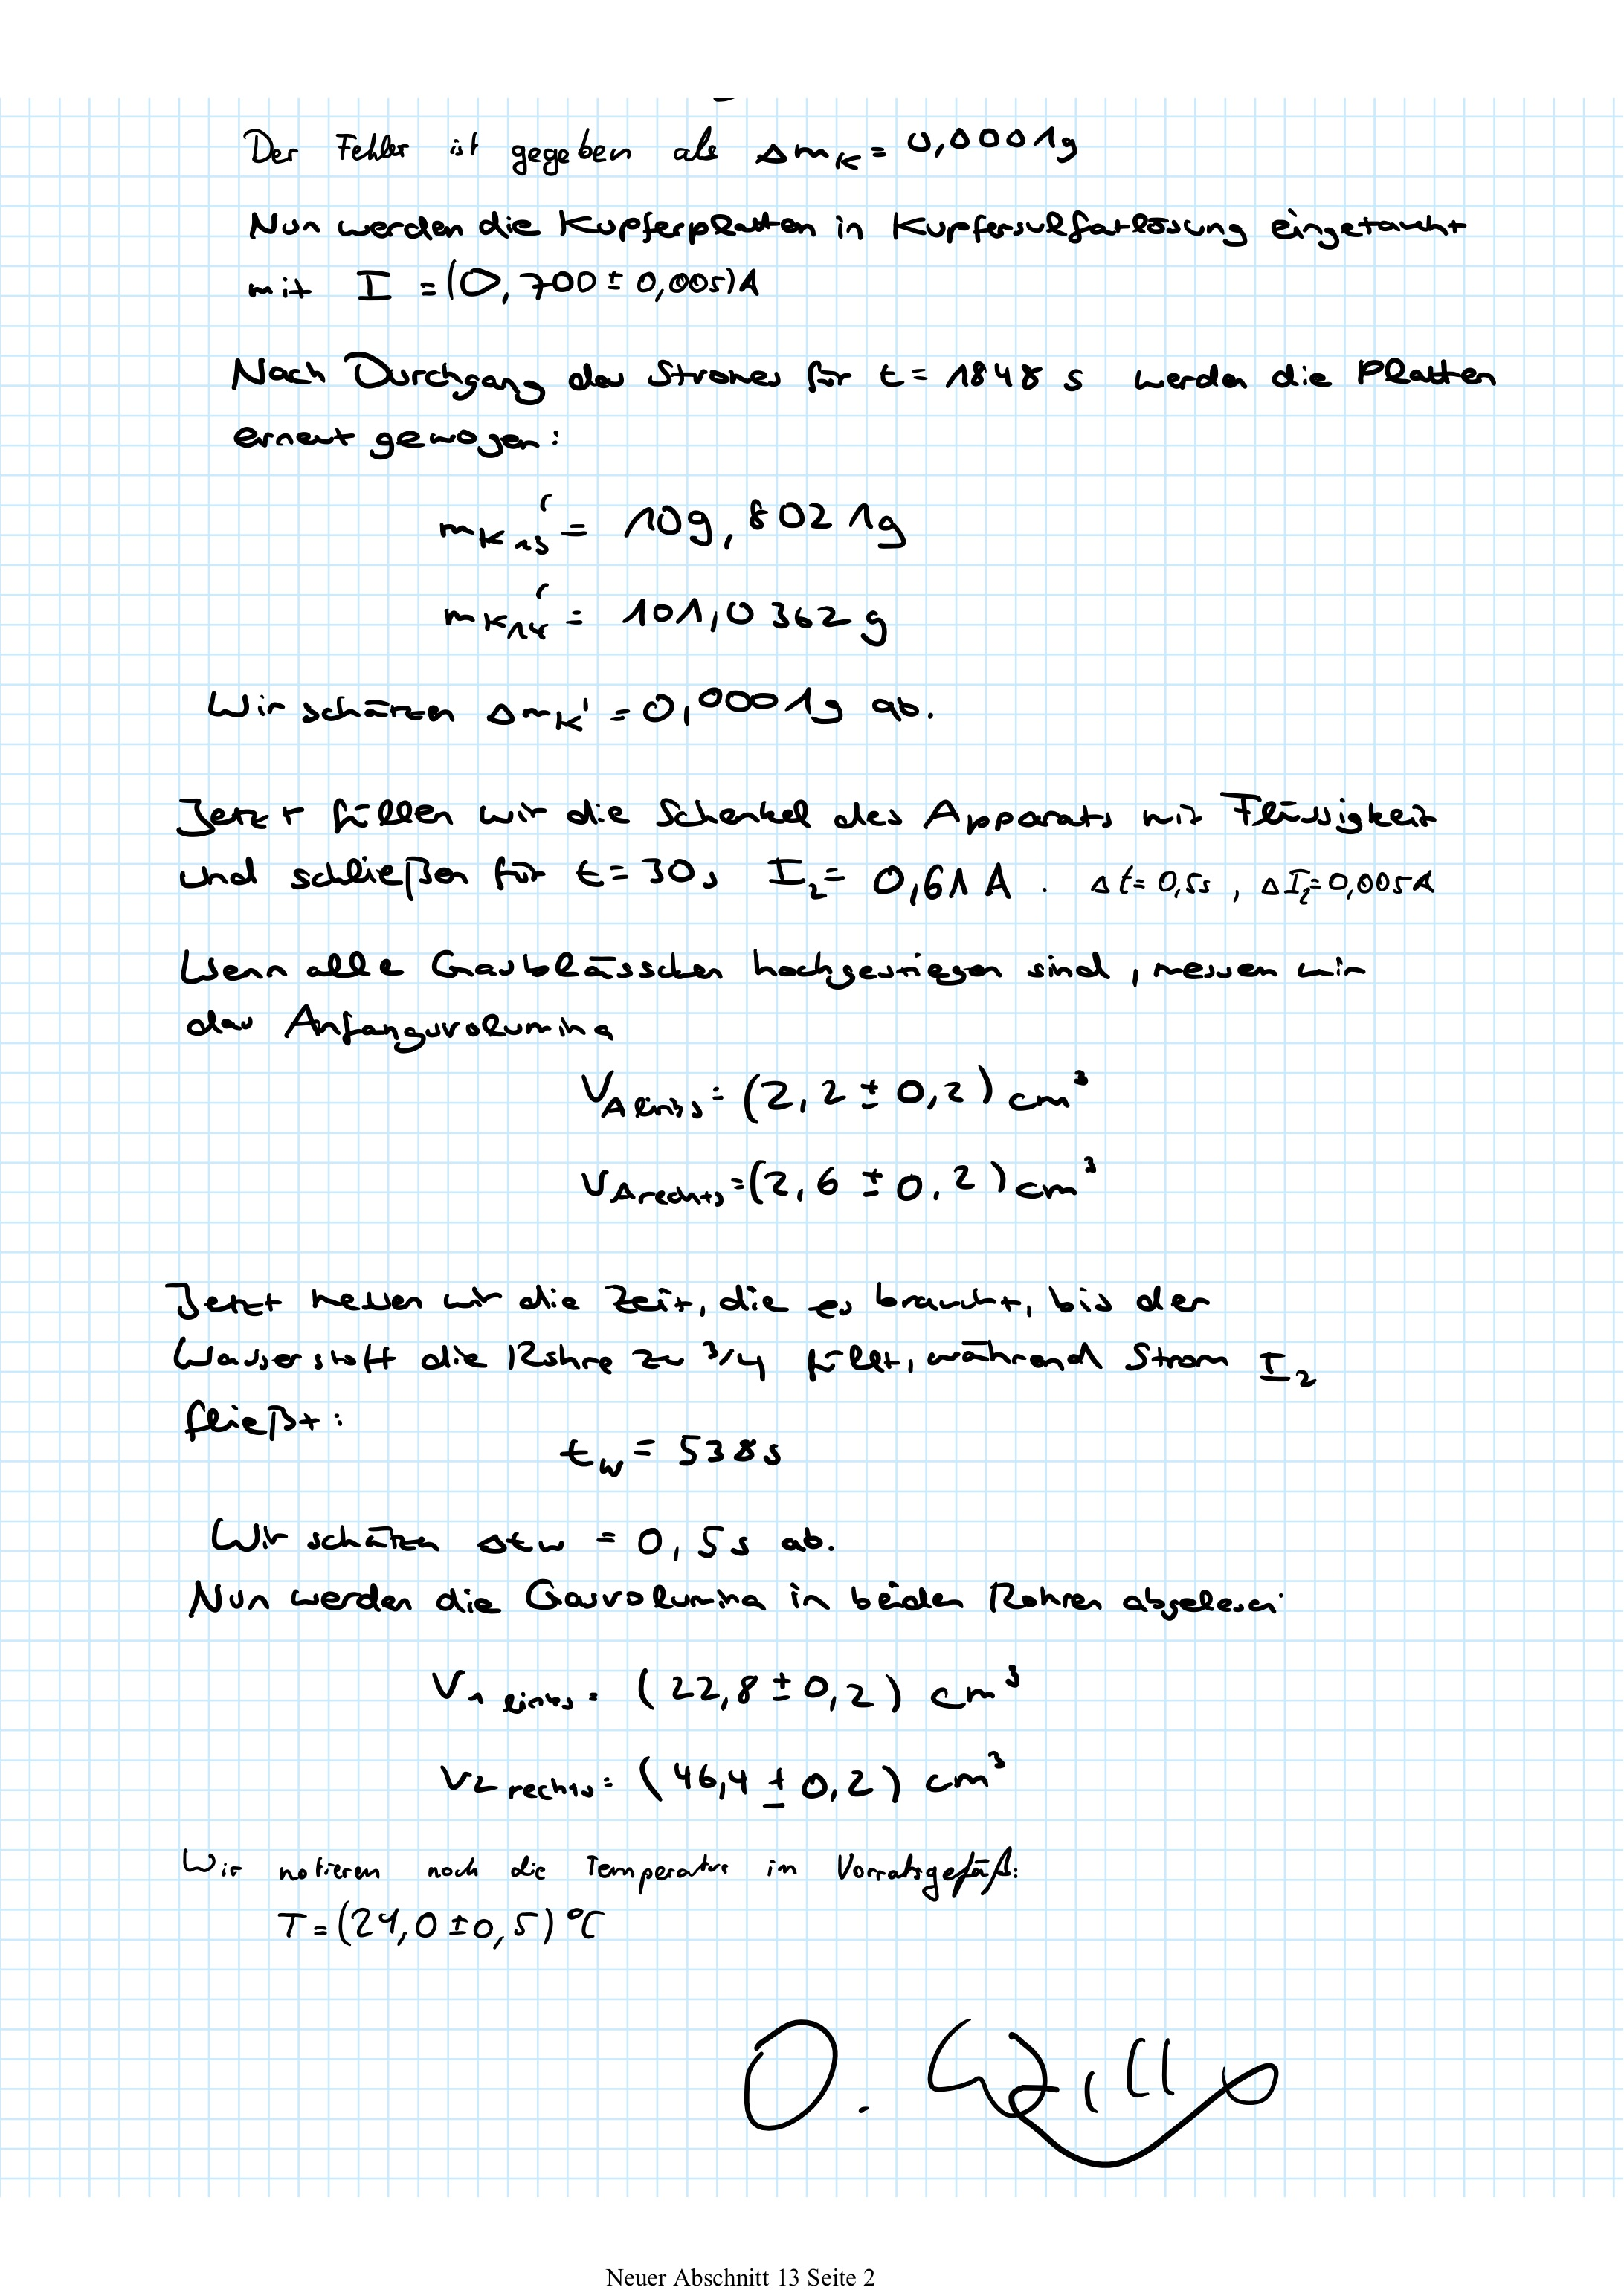
\includegraphics[width=\textwidth]{graphics/mess2.jpg}
\newpage

%-------------------------AUSWERTUNG-------------------------
\section{Auswertung}

In dieser Evaluation werden alle Fehler, sofern keine spezifische Angabe gemacht wird, mithilfe der Gauss'schen Fehlerfortpflanzung berechnet. Dies bedeutet, dass ein Wert $F$, der mit der Formel $f(a_1, ..., a_n)$ berechnet wird, den Fehler $\Delta F$ gegeben über folgende Formel hat:

\begin{equation}
    \Delta F = \sqrt{\sum_n \left( \frac{\partial f}{\partial a_n} \cdot \Delta a_n \right)^2}.
\end{equation}

\subsection{Bestimmung der Faraday-Konstante mit Massen}

Zunächst berechnen wir den Gesamtstrom $Q$ mittels Gleichung \ref{eq:Q}, der durch die beiden Kupferplatten über die Versuchsdauer $t=(1848,0\pm0,5)$s floss:

\begin{equation}
    \begin{split}
        Q = It, \ \ \ \ \Delta Q &= \sqrt{\left( I \cdot \Delta t \right)^2 + \left( t \cdot \Delta I \right)^2} \\ \\
        Q = (1294 \pm 9) \text{C}
    \end{split}
    \label{res:Q}
\end{equation}

Nun berechnen wir die beiden Massedifferenzen, wobei der Index $A$ für die Anode und $K$ die Kathode steht:

\begin{equation}
    \begin{split}
        M = |m' & - m|, \ \ \ \ \Delta M = \sqrt{2*(\Delta m)^2} \\ \\
        M_A &= (0,46390 \pm 0,00014) \text{g} \\
        M_K &= (0,43200 \pm 0,00014) \text{g} \\ %wird weniger
    \end{split}
    \label{res:masses}
\end{equation}

Die Werte für die Wertigkeit $z$ und die Molmasse $M_{Mol}$ von Kupfer sind fest und ergeben sich aus der Reaktionsgleichung \ref{eq:elektrolyse1} beziehungsweise den Eigenschaften des Stoffs. Es gilt $z = 2$ und $M_{Mol} = 63,54 \frac{\text{g}}{\text{mol}}$. 

Nun kann die Faraday-Konstante mit Gleichung \ref{eq:masse} bestimmt werden, einmal für die Massezufuhr der Anode und einmal die Masseabnahme der Kathode:

\begin{equation}
    \begin{split}
        F &= \frac{QM_{Mol}}{zM}, \\
        \Delta F &= F \sqrt{\left( \frac{\Delta Q}{Q} \right)^2 + \left( \frac{\Delta M}{M} \right)^2} \\ \\
        \bm{F_A} &= \bm{(8,86\pm 0,06) \cdot 10^{4} \frac{\textbf{C}}{\textbf{mol}}} \\
        \bm{F_K} &= \bm{(9,52 \pm 0,07) \cdot 10^{4} \frac{\textbf{C}}{\textbf{mol}}} \\
    \end{split}
    \label{res:Fm}
\end{equation}

Vergleicht man diese Werte miteinander mithilfe eines Signifitanztests, so ergibt sich:

\begin{equation}
    \sigma_{AK} = \frac{|F_A - F_K|}{\sqrt{(\Delta F_A)^2 + (\Delta F_K)^2}} = 7,16
\end{equation}

Zusätzlich vergleicht man beide Werte auf analoge Weise mit dem gegeben Literaturwert $F = (9,648455 \pm 0,000027) \cdot 10^4 \frac{\text{C}}{\text{mol}}$:

\begin{equation}
    \begin{split}
        \sigma_{AL} &= 13,14 \\
        \sigma_{KL} &= 1,84 \\
    \end{split}
\end{equation}

Die beiden Werte größer als 3 weisen signifikante Abweichung auf, der letzte Wert ist somit eine insignifikante Abweichung.

\newpage

\subsection{Bestimmung der Faraday-Konstante mit Volumina}

Erneut berechnen wir zunächst die Elektrizitätsmenge $Q$, dies geschieht analog zu Gleichung \ref{res:Q}:

\begin{equation}
    Q = (328,2 \pm 2,7) \text{C}
\end{equation}

Wir nutzen Gleichung \ref{eq:druck}, um den im Gefäß herrschenden Druck $p$ zu bestimmen. Da eine Temperatur von $T = (24,0 \pm 0,5)^\circ$C im Gefäß herrschte, übernehmen wir den Wert $p_D = 22,38$ Torr $\approx 29,8$mbar aus der im Skript gegebenen Tabelle. Wir schätzen den Fehler $\Delta p_D = 1,8$mbar aus der Tabelle ab.

\begin{equation}
    \begin{split}
        \Delta p &= \sqrt{(\Delta p_L)^2 + (0,9 \cdot \Delta p_D)^2} \\ \\
        p &= (982,5 \pm 1,6) \text{mbar}
    \end{split}
\end{equation}

Anschließend nutzen wir Gleichung \ref{eq:Vmol}, um das Molvolumen $V_{Mol}$ bei der gegebenen Gefäßtemperatur und dem gegebenen Druck auszurechnen. Wir verwenden $V_{Mol}^0 = 22,414 \frac{\text{l}}{\text{mol}}$, $p_0 = 1013,25$mbar und $T_0 = 273,15$K:

\begin{equation}
    \begin{split}
        \Delta V_{Mol} &= V_{Mol} \sqrt{\left( \frac{\Delta T}{T} \right)^2 + \left( \frac{\Delta p}{p} \right)^2} \\ \\
        V_{Mol} &= (25,15 \pm 0,06) \frac{\text{l}}{\text{mol}}
     \end{split}
\end{equation}

Nun können noch die Volumendifferenzen $V_d$ bestimmt werden:

\begin{equation}
    \begin{split}
        V_d = |V' - V|, \ \ & \ \ \Delta V_d = \sqrt{(\Delta V')^2 + (\Delta V)^2} \\ \\
        V_{d_A} &= (20,60 \pm 0,28) \text{cm}^3 \\
        V_{d_K} &= (43,80 \pm 0,28) \text{cm}^3 \\
    \end{split}
\end{equation}

Somit haben wir alles um die Faraday-Konstante über Gleichungen \ref{eq:F2} zu bestimmen. Die Wertigkeit $z$ lässt sich erneut aus der Prozessgleichung in \ref{eq:elektrolyse2} als $z=2$ für Wasserstoff und $z=4$ für Sauerstoff bestimmen.

\begin{equation}
    \begin{split}
        F' &= \frac{Q}{zV} V_{Mol} \\
        \Delta F' &= F \sqrt{\left( \frac{\Delta Q}{Q} \right)^2 + \left( \frac{\Delta V}{V} \right)^2 + \left( \frac{\Delta V_{Mol}}{V_{Mol}} \right)^2} \\ \\
        \bm{F'_A} &= \bm{(10,02 \pm 0,16) \cdot 10^{4} \frac{\textbf{C}}{\textbf{mol}}} \\
        \bm{F'_K} &= \bm{(9,42 \pm 0,10) \cdot 10^{4} \frac{\textbf{C}}{\textbf{mol}}} \\
    \end{split}
\end{equation}

Erneut vergleichen wir zunächst die beiden Werte miteinander und anschließend mit dem Literaturwert:

\begin{equation}
    \begin{split}
        \sigma_{AK} &= 3,18 \\ \\
        \sigma_{AL} &= 2,32 \\
        \sigma_{KL} &= 2,28 \\
    \end{split}
\end{equation}

Die beiden Konstanten weisen also eine signifikante Abweichung voneinander auf, aber jeweils eine insignifikante Abweichung zum Literaturwert.

\newpage
%---------------PRÄSENTATION DER ENDERGEBNISSE---------------
\section{Präsentation der Endergebnisse}

In diesem Versuch wurde viermal die Faraday-Konstante bestimmt. Zweimal über die Massenmessung und zweimal über die Volumenmessung. Dabei wurden die folgenden Ergebnisse erzielt:

\begin{equation}
    \begin{split}
        \bm{F_A} &= \bm{(8,86\pm 0,06) \cdot 10^{4} \frac{\textbf{C}}{\textbf{mol}}} \\
        \bm{F_K} &= \bm{(9,52 \pm 0,07) \cdot 10^{4} \frac{\textbf{C}}{\textbf{mol}}} \\ \\        
        \bm{F'_A} &= \bm{(10,02 \pm 0,16) \cdot 10^{4} \frac{\textbf{C}}{\textbf{mol}}} \\
        \bm{F'_K} &= \bm{(9,42 \pm 0,10) \cdot 10^{4} \frac{\textbf{C}}{\textbf{mol}}} \\
    \end{split}
\end{equation}


\newpage
%---------------ZUSAMMENFASSUNG UND DISKUSSION---------------
\section{Zusammenfassung und Diskussion}

In diesem Versuch nutzten wir Elektrolyse, um die Faradaykonstante zu bestimmen. Dabei betrachteten wir zwei verschiedene Prozesse, einmal eine Kupfersulfatlösung und einmal einen Wasserzersetzungsapparat. 

Zunächst auffallend sind die recht hohen Sigmawerte der Ergebnisse. Bei beiden Versuchsteilen ergaben die zwei bestimmten Faraday-Konstanten für die Anode und Kathode immer signifikante Abweichungen mit $\sigma=7,16$ beim ersten und $\sigma = 3,18$ beim zweiten. Außerdem ergab der erste berechnete Wert über die Anode der Kupfersulfatlösung ein Sigmaabweichung von über 10, was auf einen klaren systematischen Fehler hinweist. 

Potenzielle Fehlerquellen beim ersten Versuchsteil könnten in der Wägung der Platten verbunden mit der vorherigen Reinigung liegen. Insbesondere nach dem Elektrolysevorgang mussten die Platten vorsichtig abgewaschen werden. Es kann sein, dass hierbei eventuell etwas zu viel Material ausversehen abgewaschen wurde. 

Spezifisch beim zweiten Versuchsteil könnte die Volumenmessung fehlerbehaftet sein, da es sich als etwas schwierig herausstellte, den Behälter auf eine Höhe mit dem Wasserstand in den Röhren zu bringen, was bedeuten würde, dass der hydrostatische Druck doch nicht ganz gleich Null wäre. 

Insgesamt lässt sich anmerken, dass während der Elektrolyse natürlich nicht nur die gewollten Reaktionen, sondern auch Nebenreaktionen mit anderen Stoffen abgelaufen sind. Diese waren teils durch leichte Kristallstrukturen auf den Platten nach dem Vorgang zu erkennen. Dies wäre ein systematischer Fehler, der das Ergebnis bei allen Versuchen negativ beeinflusst. 

Insgesamt lässt sich aber sagen, dass Versuchsteil Zwei bessere Ergebnisse lieferte als Versuchsteil Eins. Hier war nämlich die Sigmaabweichung der beiden Werte voneinander mit 3,18 nur leicht über der signifikanten Grenze 3 im Vergleich zu den 7,16 vom ersten Versuchsteil. Zusätzlich sind auch die Werte im Vergleich mit dem Literaturwert mit Abweichungen von 2,32 und 2,28 Sigma besser als beim ersten Versuch, wo ein Wert zwar recht genau mit 1,84 Sigma am Literaturwert liegt, der andere Wert aber die zuvor erwähnten 13,14 Sigma aufweist. Die Ergebnisse des zweiten Teils sind also stabiler und weichen nicht so stark voneinander ab. 

Was auf einem anderen Level noch ein Grund für die großen Sigmawerte ist, sind unsere relativ kleinen Fehlerwerte. Diese sind nämlich bei keinem Endwert größer als 1,5\%, was darauf schließen lässt, dass wir bei der Fehlerabschätzung wohl einige Angaben präziser ausgewertet hatten als gerechtfertigt, was im Endeffekt zu den hohen Sigmaabweichungen beigetragen hat.

Abschließend lässt sich sagen, dass trotz der genannten Komplikationen und potenziellen Fehlerquellen zumindest drei der vier berechneten Werte für die Faraday-Konstante mit prozentual kleinen Fehlern innerhalb der 3$\sigma$-Umgebung lagen und somit schlussendlich doch aussagekräftige Erbenisse erzielt werden konnten.   

\end{document}

